\chapter{Conclusions and Recommendations}
\label{chapter-conclusion}

\begin{abstract}
This study has, until now, involved three phases: 1) A review and development of key concepts, 2) A guide to the specification of three key robust decision support methods and three variations of the highly stylized lake problem, and 3) a conversation about the results of each method and model pairing and a comparison between pairings. In the first part of this final stage of the IMRAD structure, the key developments of this study will be discussed. Information from the first stages of this study will then be leveraged to answer the primary research question. 

\begin{researchquestion}{Research Question}
    What are the trade-offs between different methods of decision support when considering a wicked problems and varying policy implementation structures?
\end{researchquestion}

\end{abstract}

\newpage

\section{Process and Developments}
This first section will address the sub-questions that were developed in support of the primary research question in the original research definition. The structure of this section will follow that of the identified sub-questions, found in \cref{def-supporting-questions}. Each sub-question will be repeated as it is discussed for ease of reference. 

    \subsection{Key concepts}
    The first set of sub-questions identified in the research definition are addressed as key concepts in \cref{chapter-review} and are answered below. 
        
        \subsubsection{Robustness}
        \textit{How is robustness defined in policy analysis? }
        
        Robustness has been used in system and policy analysis as an alternative to address existing problems with a search for the optimal solution: the difficulties of precisely defining a model of the system under consideration and of balancing conflicting objectives, and the potential for catastrophic failure if the conditions required for an optimal solution are not maintained. A robust policy has been defined as one that performs well across a variety of possible future states of a system, due to both internal and external changes.
        
        A review of previous uses of robustness in policy analysis revealed a large variety of mechanisms that can be used to measure a policy's robustness. Selection of an appropriate robustness metric is a choice that decision makers and anlysts must make together, based on their threshold for risk and guided by the data provided by an analysis to assess robustness. 
        
        \subsubsection{Robust decision support methods}
        \textit{What are the origins of each of the selected robust decision support methods?}
        
        Through a review of previous literature on optimization and decision making under conditions of deep uncertainty, a generalized structure for a robust decision support framework was developed. The robust decision support methodology as described in this research originated as the robust decision making (RDM) method, which provided way to analyze wicked problems that are deeply uncertain in a structured manner. This early framework provided clear mechanisms for model specification, computational experimentation, and scenario discovery, but did not provide much guidance for specifying policy alternatives that properly balance conflicting objectives. Given that wicked and deeply uncertain problems will always include disagreements among involved decision makers and conflicting objectives, establishing a list of policy alternatives that will provide the highest potential for system robustness and balance the requirements of those conflicting objectives can be extremely difficult. 
        
        To address this gap in RDM, an extension was developed known as MORDM. This was one of the first commonly applied instances of the integration of a multi-objective search for policy alternatives into decision support analysis. The search in MORDM selects policy alternatives based on performance in a single reference scenario. Other extensions of the RDM framework have built on the work of MORDM and attempt to incorporate robustness more and more directly into the multi-objective search. Multi-scenario MORDM does this by using multiple independent reference scenarios across multiple repetitions of the multi-objective search to provide a more diverse mechanism with which to evaluate performance of a policy alternative. MORO, developed into a robust decision support framework in this study, goes even farther by evaluating policy alternatives based on their robustness over a small set of policies. 
        
        These three frameworks are based on the fundamental RDM structure and all use a multi-objective search for policy alternatives. Visual descriptions of the three methods are shown in \cref{fig:diff-flows-conclusion} and provide a clear communication of how each uses and customizes the RDM structure. 
                
        \begin{figure}[h]
            \centering
            \captionsetup{justification=centering}
            
            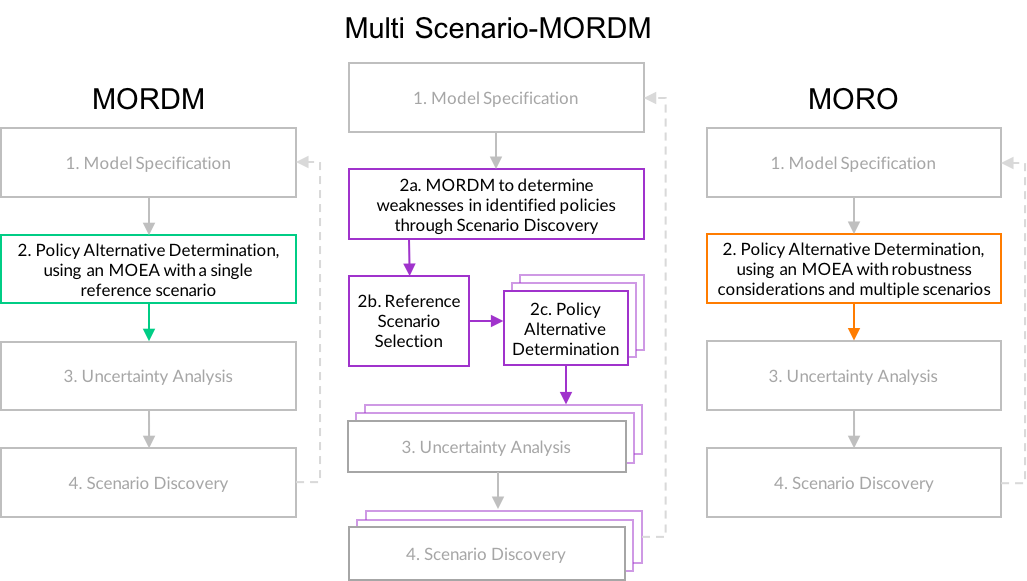
\includegraphics[width=\textwidth]{diff-flows}
            \caption{Comparison of robust decision support framework structures}
            \label{fig:diff-flows-conclusion}
        \end{figure}
    
        \cref{fig:diff-flows-conclusion} highlights the large similarities held by each of the three methods. In fact, steps 1, 3, and 4 are common for all three methods. The difference in methods exists only in step 2: policy alternative determination. And in this step, as described in \cref{dev-step2}, each method uses the same basic multi-objective search algorithm and instantiation of that algorithm, with the differences being concentrated in the mechanism the algorithm uses to compare policy alternatives. By limiting methodological differences to such a small piece of each method, any differences uncovered in this study will be more easily attributable to that single point of difference, providing a stronger foundation for comparison. 
                
        \subsubsection{Evaluating RDM frameworks}
        \textit{How have stylized policy problems been leveraged in previous research?} \newline
        \textit{How does the lake problem incorporate deep uncertainty tipping point behavior?}
        
        To evaluate the performance of each RDM framework against wicked problems with tipping point characteristics, a commonly used stylized problem will be employed: the lake problem. As problems that involve a tipping point generally contain high levels of uncertainty, a point of no return, and conflicting objectives, they are recognized as strong candidates to evaluate decision support frameworks \citep{Ward2015}. The lake problem is a classic tipping point problem that has been used frequently to develop and evaluate robust decision support frameworks \citep{Carpenter1999, Lempert2007, Quinn2017, Singh2015, Ward2015}. The lake problem revolves around a fictional town that is seeking to maximize economic productivity of industry and agriculture through the release of pollution, while at the same time to minimize risk of over-pollution of a nearby lake, represented as a series of four conflicting objectives. 
        
        \textit{What policy implementation structures are commonly recognized in literature?}
        
        Two different variations of the lake problem have been previously developed that represent extremes of static and adaptive policy structures. The intertemporal variation requires policies to use a set of predetermined decisions that define the pollution release level at every time step \citep{Ward2015}. And the direct policy search variation uses decision levers to build a release function that incorporates current pollution levels and is used to set the pollution release level every time step \citep{Quinn2017}. 
        
        Both the intertemporal and DPS policy structures include the ability to alter the amount of anthropogenic pollution release in every time step, which does not reflect typical real world conditions, where such a change often requires significant investment and decision making moves more slowly. A planned adaptive DPS variation of the lake problem was proposed that follows the policy implementation structure of the DPS variation, but updates the release amount every 10 time steps to more accurately reflect policy structure that is found in real world decision making. 
    
    \subsection{Methodology}
    Similar to the key concepts, the next section will address the methodological sub-questions developed as a part of the research definition. The methodology applied in this study was developed in \cref{part-develop}. 
        
        \subsubsection{Lake Problem Variations}
        \textit{What are definitions of the lake problem that represent the three essential types of policy implementation?}
        
        The intertemporal and DPS variations of the lake problem were implemented following the details of previous applications in literature \citep{Kwakkel2017, Quinn2017, Singh2015, Ward2015}. The proposed planned adaptive DPS variation follows the implementation structure of the DPS lake problem, but only refreshes the pollution release amount every 10 time steps instead of at every time step, as is done in the traditional DPS variation. No changes to any of the model variations were required across all three methods of analysis. This, again, limits the differences being considered and ensures a more fair comparison. 
        
        \subsubsection{Method Implementation}
        \textit{How can robustness be determined for each selected robust decision support method?} 
        
        A common robustness definition was used for all three robust decision support methods: Starr's domain criterion \citep{Starr1963}. The exact implementation of this metric was described in \cref{dev-step0}, including a definition of the outcomes of interest and threshold values that are based on previous applications of the lake problem \citep{Quinn2017, Ward2015}. Using a common robustness definition minimizes the differences between method and model variation pairings and allows for a straightforward comparison of results between the three robust decision support methods. 
        
        \textit{What are the implementation details for each robust decision support method identified for this study?}
        
        Further details of each method implementation are found in \cref{dev-step2}. Most notably, an auto-adaptive variation of the $\epsilon$-NSGAII algorithm was developed that combines an epsilon-based multi-objective search using techniques developed by \citet{Deb2002} with auto-adaptive operator selection introduced by \citet{HadkaReed2013} and previously used in the Borg framework. This auto-adaptive $\epsilon$-NSGAII algorithm aims to combine the strongest points of $\epsilon$-NSGAII, a generational MOEA with epsilon dominance, and Borg, which supports auto-adaptive operator selection and auto-adaptive population sizing, to allow for a more rapid convergence to a stable set of non-dominated policy alternatives. The same auto-adaptive $\epsilon$-NSGAII algorithm is used for all three methods in this study, with a common parameterization. The only difference lies in the mechanism used to compare potential policy alternatives during the search process, with each method using their own unique mechanism. These mechanisms were described in \cref{step2-scenarios} and are summarized in \cref{table:conclusion-searchevaluation}. The inclusion of robustness provides a indication of how much robustness was included in the search phase for each method relative to the other methods considered. It is by no means an absolute indication of the inclusion of robustness for each method. 
        
        \begin{table}[H]
            \centering
            \captionsetup{width=\textwidth}
            \caption{Policy alternative comparison mechanism used in the MOEA-based search for each method.}
            \label{table:conclusion-searchevaluation}
            
            \setlength\arrayrulewidth{1pt}\arrayrulecolor{white}
            \rowcolors{2}{odd-row-blue}{even-row-blue}
            \begin{tabularx}{\textwidth}{|l|X|l|}
                \rowcolor{tudelft-dark-blue!80}
                {\color{white} Method} &  {\color{white} Comparison Mechanism} & {\color{white} Inclusion of Robustness} \\ \hline
                
                MORDM & Absolute performance in single base reference scenario & Low \\ \hline
                Multi-Scenario MORDM & Absolute performance in one of a set of reference scenarios, with search repeated for each scenario & Medium \\ \hline
                MORO & Robustness score calculated using a small set of (50) scenarios & High \\ \hline
            \end{tabularx}
        \end{table}
        
        Details of the comparison mechanism for MORDM are quite straightforward, using a single base reference scenario. The multi-scenario MORDM method requires a clear definition of how the set of reference scenarios used is determined. In this case, a set of four scenarios are selected that are maximally diverse within vulnerable ranges identified in MORDM's scenario discovery step. Finally, the MORO method involved defining a constant set of 50 scenarios with which to test each possible policy alternative. Alternatives are then added to the non-dominated set of policy alternatives based on the robustness of each outcome of interest. Robustness is calculated using the established domain criterion metric and thresholds from \cref{dev-step0}. 
        
        In addition to the details established for each method's policy alternative determination step, \cref{dev-step3} and \cref{dev-step4} defined mechanisms for uncertainty analysis and scenario discovery that are shared across all three robust decision support methods and follow the implementation established when the MORDM method was introduced \citep{Kasprzyk2013}. 
        
        \subsubsection{Comparison Specification}
        \textit{What are the points of comparison which should be considered during analysis?}
        
        Existing literature that compare methods for policy analysis were examined to develop a comprehensive set of 11 comparison metrics. This set of metrics serves two purposes. First, to provide a strong and common foundation for future comparisons of policy analysis methods. Second, to establish the metrics with which to compare the three robust decision support methods considered in this study. These metrics include both qualitative and quantitative measures and were divided into three categories: setup complexity, communication, and results. Metrics include complexity of problem and method setup, ease of results communication and response to change, computational cost, robustness of policies, and similarity of results and robustness. Details of each metric are discussed in \cref{dev-comparisons}. 
                
    \subsection{Results}
    The final group of sub-questions address the results of each method and model variation pairing, along with the comparisons made. A detailed analysis of the results was included as \cref{part-analysis}. 
    
        \subsubsection{Individual Results}
        \textit{What are the results from each pairing of robust decision support method and variation of the stylized policy problem?}
        
        Considering the results of each method variation and method pairing separately provides the foundation for a comparative analysis by establishing the validity of each pairing before attempting any direct comparisons. These individual results were discussed in \cref{analysis-results}. The results showed that the MOEA search for each pairing stabilized successfully to a promising set of policy alternatives. The uncertainty and scenario discovery results were also summarized in \cref{analysis-results}. 
        
        %TODO EEB compare results to existing analysis (Quinn, Wade, etc. )
        
        \subsubsection{Comparison of Results}
        \textit{Based on the points of comparison defined in \cref{dev-comparisons}, how do the results of each pairing compare?}
        
        After the individual results were examined and validated, a comparison was made. Using the metrics defined in \cref{dev-comparisons}, \cref{chapter-comparison} compared the various method and model variation pairings. This section summarizes the key findings made during comparison and is divided into three categories, following the structure established with the comparison framework in \cref{dev-comparisons}. 
        
        \textbf{Setup} \newline
        With respect to problem complexity, each method is able to use the same implementation of each lake problem variation, so there is no difference in setup. 
        
        Method setup complexity includes some variable differences. Given the method implementations used for this study, the setup of multi-scenario MORDM requires a complete MORDM analysis and extensive additional computation to determine a maximally diverse set of reference scenarios, so setup is significantly more complicated than it is for the other two methods. It is important to note that the complexity of setup for multi-scenario MORDM can be reduced by using a different mechanism to build the set of reference scenarios than is used in this study.
        
        \textbf{Communication} \newline
        Each method is able to use the same definition of robustness and builds final results with the same processes of policy alternative determination, uncertainty analysis, and scenario discovery, so there is no difference in the communication of results or robustness for this study. 
        
        The common implementations for the final two steps in the RDM flow also mean that there is no significant difference in the updating the results of those two stages if the model or robustness metric changes. One exception lies in the impact of a change in robustness metric to the policy alternative determination process for MORO-based analyses. Because MORO directly integrates robustness into the search process, an update to the metric will require a restart of the policy alternative determination process. 
        
        \textbf{Results} \newline
        MORO requires significantly higher computational cost, given that each potentially promising policy alternative must be evaluated over 50 scenarios and not just one. With that cost, though, comes a generally smaller and more robust set of non-dominated alternatives than what is found with the other two methods. The robustness of each set of non-dominated policy alternatives indicate that the more robust considerations are incorporated into the search process, the higher the robustness of the final non-dominated set of alternatives will be. This is seen in the heatmap of mean robustness values for each method and model variation pairing that was included in \cref{results-compare-results} and is reproduced here as \cref{fig:conclusion-robust-heatmap-mean} for ease of reference.
        
        The exception to the general rule of increasing robustness can be seen with the results of the planned adaptive DPS model variation. A sharp increase in robustness with respect to pollution level and reliability was found in the multi-scenario MORDM analysis of the planned adaptive DPS variation that was not seen with the other two variations. A likely cause lies in the set of recommended policies for that pairing, which were much more conservative with respect to the amount of pollution released in each time step. The set of non-dominated policies for this pairing were also found to lead to a less diverse set of robustness outcomes, with most of the policies yielding high robustness with respect to pollution and reliability and lower robustness with respect to utility (as displayed in \cref{fig:perpolicy-robustness}).
        
        These facts together demonstrate the significant impact that the reference scenario selection process can have during a multi-scenario MORDM analysis, which can lead to results that prioritize one outcome of interest over another. Because it is impossible for problems characterized by deep uncertainty to include a consistent ranking of the preference of outcomes of interest, such a prioritization of one outcome in the policy alternative determination process should be avoided wherever possible.
        
        Additional study of the planned adaptive DPS model variation and multi-scenario MORDM pairing was completed that compared the results of the reference scenario selection method applied in this study with a random scenario selection. Robustness results using random scenario selection produced values similar to what was found with the traditional MORDM analysis, which adds emphasis to the importance of reference scenario selection on the analysis process. Given that the same mechanism is used to select reference scenarios for all three problem variations, there are also indications that the slower moving policy structure found in the planned adaptive DPS variation is more susceptible to strong influences from the selection of reference scenarios. 
      
        \begin{figure}[H]
            \centering
            \captionsetup{width=0.8\textwidth}
            
            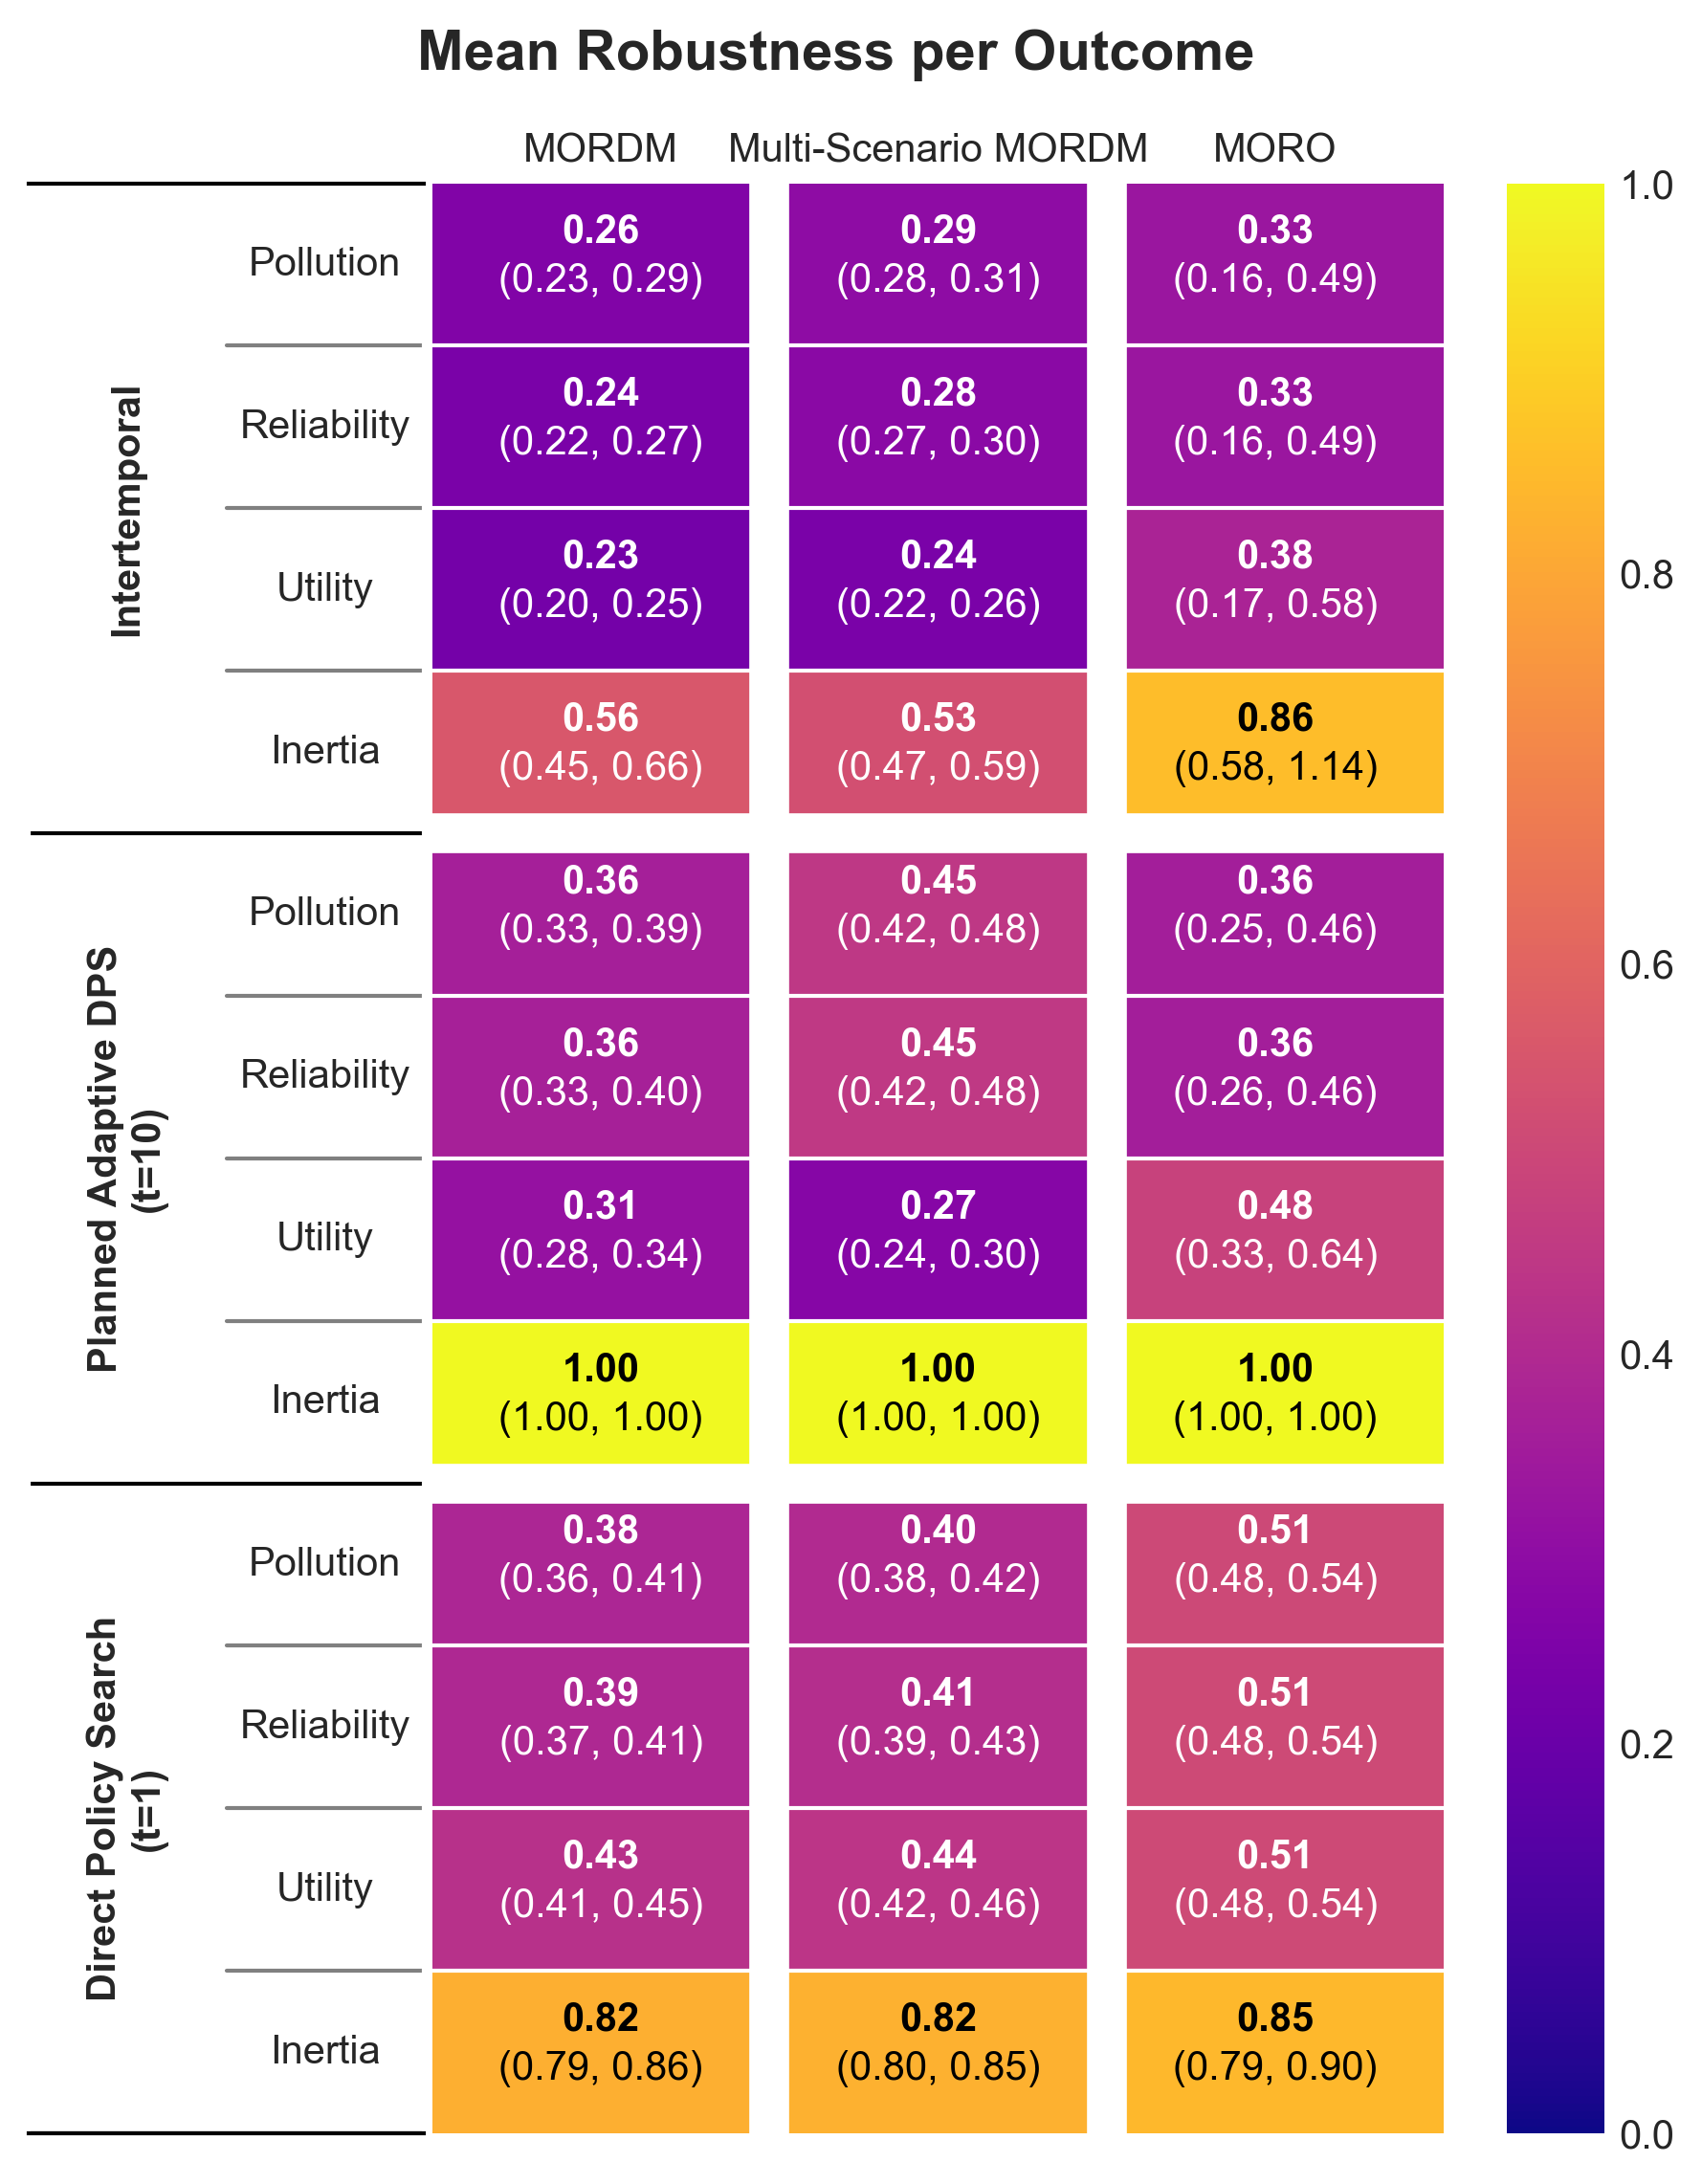
\includegraphics[width=0.8\textwidth]{compare/robust_heatmap_mean}
            \caption[Mean robustness per outcome of interest across all pairings]{Mean robustness per model variation and method pairing. This heat map is annotated to include the bounds of the 95 percent confidence interval surrounding the mean.}
            \label{fig:conclusion-robust-heatmap-mean}
        \end{figure}
              
\section{Answering the Primary Research Question}
The answers to each sub-question can now be used to answer the primary research question, repeated here. 

\begin{researchquestion}{Research Question}
    What are the trade-offs between different methods of decision support when considering a wicked problems and varying policy implementation structures? 
\end{researchquestion}

The categorization of each point of comparison considered in this analysis provide a structure for considering trade-offs that exist when determining which robust decision support method to use in an analysis of a wicked policy problem with tipping point characteristics. In this study, the first category, setup complexity, provides little guidance to distinguish the three methods, as each was executed using the same software tooling and has the same requirements for model implementation. Of course, as discussed in \cref{dev-step0}, there are other packages that support the policy analysis process as well that are not able to support all three analysis methods. In that case, there may be significant differences in the setup complexity for both the model and method being used. 

The second category, communication and interaction, provides some stronger trade-offs between methods. The MORDM method is least affected by changes in model or robustness specification. A change in robustness metrics during an MORDM-based analysis would only require recalculation of the robustness values of each policy alternative using an already completed ensemble of computational experiments. A change in robustness metric configuration may require a restart of part, in the case of multi-scenario MORDM, or all, in the case of MORO and multi-scenario MORDM, of the policy alternative determination process. Therefore, if the configuration of a robustness metric is more likely to change during the course of an analysis, decision makers may be more interested in an MORDM-based analysis. 

The final category of comparison metrics provides the most opportunity for differentiation between methods. As indicated by \cref{table:conclusion-computational-cost}, a MORO analysis has a significantly higher computational cost than for the other robust decision support methods. The increased computational cost had a significant impact on the time it took to complete the analysis even for a highly-stylized and relatively low computational cost problem like the lake problem used in this analysis and can have an even more significant impact when considering policy problems that require significantly more complex models with more sources of uncertainty than are present in the lake problem. 

\begin{table}[b!]
    \captionsetup{width=0.99\textwidth}
    \caption[Computational cost across all pairings]{Computational cost of the MOEA-based search determined for each model variation and method pairing. Total computational cost, calculated as number of model function executions, can be found in the last row.}
    \label{table:conclusion-computational-cost}
    
    \rowcolors{2}{odd-row-blue}{even-row-blue}
    \setlength\arrayrulewidth{1pt}\arrayrulecolor{white}
    \begin{tabularx}{0.99\linewidth}{l|l|R|R|R}
        \hline
        \rowcolor{tudelft-dark-blue!80}
        \multicolumn{2}{l|}{\color{white} \textbf{}} 
        & \multicolumn{1}{c|}{\color{white} \textbf{MORDM}} 
        & \multicolumn{1}{c|}{\color{white} \textbf{\begin{tabular}[c]{@{}c@{}}Multi-\\ Scenario \\ MORDM\end{tabular}}}
        & \multicolumn{1}{c}{\color{white} \textbf{MORO}} \\ \hline
        
        \cellcolor{even-row-blue}   & Intertemporal    & 500,000   & 500,000  &  300,000    \\ \cline{2-5} 
        \cellcolor{even-row-blue}   & \cellcolor{odd-row-blue}Planned Adaptive &
        \cellcolor{odd-row-blue}100,000   & \cellcolor{odd-row-blue}100,000  & \cellcolor{odd-row-blue}100,000     \\ \cline{2-5} 
        \multirow{-3}{*}{\cellcolor{even-row-blue}\begin{tabular}[c]{@{}l@{}}Number of \\ Function \\ Executions (NFE)\end{tabular}} & DPS             & 100,000   & 100,000  & 100,000      \\ \hline
        
        \multicolumn{2}{l|}{\cellcolor{odd-row-blue}Per Policy Executions} & 1 & 1 & 50 \\ \hline
        \multicolumn{2}{l|}{\cellcolor{even-row-blue}Search Repetitions} & 1 & 5 & 1 \\
        
        \noalign{\global\arrayrulewidth=4pt} \arrayrulecolor{tudelft-dark-blue!80}
        \hline
        \noalign{\global\arrayrulewidth=1pt} \arrayrulecolor{white}
        
        \cellcolor{odd-row-blue}    
        & \textbf{Intertemporal}    & 500,000  & 2,500,000 & 15,000,000  \\ \cline{2-5} 
        \cellcolor{odd-row-blue} 
        & \cellcolor{even-row-blue}\textbf{Planned Adaptive} & \cellcolor{even-row-blue}100,000  & \cellcolor{even-row-blue}500,000   & \cellcolor{even-row-blue}5,000,000    \\ \cline{2-5} 
        \multirow{-3}{*}{\cellcolor{odd-row-blue}\textbf{\begin{tabular}[c]{@{}l@{}}Computational \\ Cost (NFE) \end{tabular}}}      
        & \textbf{DPS}              & 100,000  & 500,000   & 5,000,000           \\ \hline
    \end{tabularx}
\end{table}

Contrasted with computational cost is the robustness of each recommended set of non-dominated policy alternatives. As highlighted earlier in this chapter, the robustness of a non-dominated set of alternatives is generally seen to increase as the consideration of robustness in the search process increases. The trade-off then becomes one between robustness of the recommended set of policy alternatives and computational cost of analysis, where decision makers who are able to sacrifice time and computational cost and who are interested in the most robust options may desire a MORO-based analysis, and decision makers who are unable to spend the additional computational cost may prefer a MORDM-based analysis. A multi-scenario MORDM-based analysis can provide a middle path between the two extremes of MORDM and MORO, but issues of setup complexity and the impact of reference scenario selection may outweigh the benefits of a small amount of added robustness obtained with multi-scenario MORDM.

Also worth consideration is the size of each set of non-dominated policy alternatives, summarized in \cref{table:conclusion-pareto-size}. Both MORDM and multi-scenario MORDM based analyses lead to a significantly larger number of non-dominated policies that must then be considered throughout the remaining steps of analysis. Methods that recommend larger sets of policy alternatives can prove to be more difficult for decision makers to digest in order to reach a final plan of action. 

At the same time, consideration of a larger set of policy alternatives can provide a more diverse set of options for decision makers to chose from, providing more opportunity to determine how best to balance conflicting objectives through discussion and debate after an a priori analysis has been completed with as minimal an influence from decision makers as possible. This represents the final trade-off discussed as a part of this study. Decision makers who are interested in a small set of robust policy options may prefer a MORO-based analysis, while decision makers who are more interested in a large and diverse set of alternatives to consider further may prefer either an MORDM or multi-scenario MORDM-based analysis. 

\begin{table}[h]
    \centering
    \captionsetup{width=0.85\textwidth}
    \caption[Size of non-dominated policy alternative sets]{Size of the Pareto non-dominated set of policy alternatives for each model variation and method pairing.}
    \label{table:conclusion-pareto-size}
    
    \rowcolors{2}{odd-row-blue}{even-row-blue}
    \setlength\arrayrulewidth{1pt}\arrayrulecolor{white}
    \begin{tabularx}{.85\linewidth}{l|R|r|R}
        \rowcolor{tudelft-dark-blue!80}
        & \multicolumn{1}{c|}{\color{white} \textbf{MORDM}}
        & \multicolumn{1}{c|}{\color{white} \textbf{Multi-Scenario MORDM}}
        & \multicolumn{1}{c}{\color{white} \textbf{MORO}} \\ \hline
        
        Intertemporal       & 90    & 291   & 7     \\ \hline
        Planned Adaptive    & 48    & 113   & 6     \\ \hline
        DPS                 & 110   & 209   & 22    \\ \hline
    \end{tabularx}
\end{table}
